\documentclass[11pt,a4paper]{article}

% These are extra packages that you might need for writing the equations:
\usepackage{amsmath}
\usepackage{amsfonts}
\usepackage{amssymb}
\usepackage{booktabs}
\usepackage{hyperref}
\usepackage{listings}
\usepackage{xcolor}

% You need the following package in order to include figures in your report:
\usepackage{graphicx}

% With this package you can set the size of the margins manually:
\usepackage[left=2cm,right=2cm,top=2cm,bottom=2cm]{geometry}


\begin{document}

% Enter the exercise number, your name and date here:
\noindent\parbox{\linewidth}{
 \parbox{.25\linewidth}{\large HPCSE, HW 6}\hfill
 \parbox{.5\linewidth}{\begin{center} \large Beat Hubmann \end{center}}\hfill
 \parbox{.2\linewidth}{\begin{flushright} \large May 31, 2019 \end{flushright}}
}
\noindent\rule{\linewidth}{2pt}

\section{Task 1: Heat2D on MPI}

Initial remark: An attempt at solving the full task including subtasks c) and d) was made but
time was not sufficient to eradicate bugs in subsections c) and d) for multgrid. Hence,
the code is submitted as-is with partially functioning multigrid kernels which are
deactivated by setting the gridCount to 1.
\\

\subsection{Implementation}
The original code was refactored and extended to include the following:
\begin{itemize}
	\item storing all grids in \texttt{double*} pointers instead of the original cumbersome \texttt{double**} pointers.
	\item extending \texttt{gridLevel} to hold MPI-specific information
	\item extending each level's grids to include halos for MPI communication
	\item introducing a new \texttt{world} struct for each MPI rank to hold grid-specific information
	\item using \texttt{MPI\_Cart\_create} and associated MPI calls to dynamically create a cartesian grid
\end{itemize}

\subsection{Results}
The CPU code was run as-is for a baseline reference.\
The MPI code was run for a single rank and then for 1, 2 and attempted 4 full nodes.\
Unfortunately, the production version of the code without any print statements slowing
down the execution was only submitted on the morning of May 31, 2019 after loss
of Euler priority privileges. This meant that 4 node jobs could no longer be submitted and also
that all but one of those jobs were still pending the evening of May 31 after having sat 
in the queue for 10+ hours.\
Switching all jobs over to Daint at that point in time was not realistic, but 
limited functional but non-representative experiments on a smaller grid were conducted on my own machine.\
All outputs obtained are given in appendix A.

\subsection{Discussion}
All runs exhibit the same L2Norm as required in the task specification.
The strong scaling speed-up and efficiency are observed as follows.

\subsubsection{Jacobi smoothing}
\begin{itemize}
	\item 24 threads: Speed-up xxx, efficiency xxx\%
	\item 48 threads: Speed-up xxx, efficiency xxx\%
	\item 96 threads: Speed-up xxx, efficiency xxx\%
\end{itemize}
\subsubsection{Residual calculation}
\begin{itemize}
	\item 24 threads: Speed-up xxx, efficiency xxx\%
	\item 48 threads: Speed-up xxx, efficiency xxx\%
	\item 96 threads: Speed-up xxx, efficiency xxx\%
\end{itemize}
\subsubsection{L2Norm calculation}
\begin{itemize}
	\item 24 threads: Speed-up xxx, efficiency xxx\%
	\item 48 threads: Speed-up xxx, efficiency xxx\%
	\item 96 threads: Speed-up xxx, efficiency xxx\%
\end{itemize}

\subsubsection{Overall}
\begin{itemize}
	\item 24 threads: Speed-up xxx, efficiency xxx\%
	\item 48 threads: Speed-up xxx, efficiency xxx\%
	\item 96 threads: Speed-up xxx, efficiency xxx\%
\end{itemize}

As explained above, the only experiments that could be completed were on my own machine with a smaller grid, where
where the Jacobi smoothing and the residual calculation show a linear speedup and almost perfect efficiency with increasing number of ranks,
while the L2Norm kernel's efficiency decreases as ranks are added due to the collective operation of
exchanging local L2Norms.

Looking at the overall efficiency it would be expected that commmunication costs
increase and efficiency decreases as we add ranks on multiple nodes. Optimizing communication could
help with this to some extent, but ultimately the algorithm as-is suffers from having to 
perform an \texttt{MPI\_Allreduce} for each rank to decide when to stop iterations.



\section{Task 2: Communication-Tolerant Programming}



\subsection{Part a)}
\subsubsection{Implementation}
Using OpenMP, the first hybrid model can be implemented by adding the line
\texttt{\#pragma omp parallel for collapse(3)} before calculating the Jacobi stencil.
This can be done because the loops are perfectly nested and no data race is created.\
Further, as discussed on Piazza, the grid parameter was changed to 768 to allow for
integer divisibility by the required number of ranks.

\subsubsection{Results}
Strangely, the L2 Norms achieved were somewhat inconsistent even though the directive
of adapting the grid size to 768 given on Piazza was adhered to. This applies also
to the given pure MPI code which was run otherwise unmodified.\
The pure MPI code was run as-is for a baseline reference on 1, 2 and 4 full nodes.\
The hybrid MPI/OpenMP code was run for a partial load on 1, 2 and 4 nodes
 and then for 1, 2 and 4 full nodes.\
All outputs are given in appendix B.

\subsubsection{Discussion}
Looking at the pure implementation, network communication becomes evident as expected when we
increase from 2 to 4 nodes.\
For the hybrid implementation, it was attempted to unveil communication cost by running
a partial load distributed across several nodes. The increasing significant \texttt{MPI\_Waitall} times
when the isolated MPI ranks are distributed across several nodes reflect those relevant communication cost.\
Runnig the hybrid implentation on full nodes in an attempt to reduce the requirement for communication
initially shows no improvement on 2 full nodes probably as the reduced communication between ranks
is compensated by increasing message size as the ranks' grid fractions are larger in this case.
However, when running the hybrid model on 4 full nodes, the \texttt{MPI\_Waitall} reduce by a factor of 
almost two as the benefits of less communication per se coincides with reduced message size, hinting that this
benefit would likely increase when adding further nodes.





% \begin{figure}[ht]
% 	\begin{center}
% 	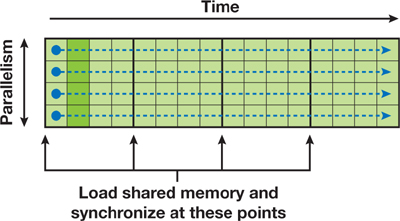
\includegraphics[scale=1.0]{tiles.jpg} 
% 	\end{center}
% 	\caption{Tiling and shared memory logic. Image credit: NVIDIA Corporation~\cite{nbody}.}
% 	\label{fig:1}
% 	\end{figure}
	


\appendix


\section{Task 1 Euler outputs}
\begin{lstlisting}[basicstyle=\tiny,
				   frame=single,
				   breaklines=true,
  	               postbreak=\mbox{\textcolor{red}{$\hookrightarrow$}\space},
				   caption={Task 2: Collected Euler outputs.}, label={lst:1}]
	
	CPU:          1 node(s) / 1 thread(s)
	-----------------------------------------------------------
	N/A (Job still in Euler queue after 12h approaching deadline on May 31)
	
	MPI:          1 node(s) / 1 thread(s)
	-----------------------------------------------------------
	N/A (Job still in Euler queue after 12h approaching deadline on May 31)
	
	MPI:          1 node(s) / 24 thread(s)
	-----------------------------------------------------------
	N/A (Job still in Euler queue after 12h approaching deadline on May 31)
	
	MPI:          2 node(s) / 48 thread(s)
	-----------------------------------------------------------
	MPI num_procs: 48
	MPI dims_x: 8
	MPI dims_y: 6
	
		Time (s)    Grid0      Total  
	-------------|---------|---------
	Smoothing    | 478.754   |  478.754  
	Residual     | 138.568   |  138.568  
	Restriction  | 0.000   |  0.000  
	Prolongation | 0.000   |  0.000  
	L2Norm       | 341.930   |  341.930  
	-------------|---------|---------
	Total        | 959.252   |  959.252  
	-------------|---------|---------
	
	Running Time      : 20.232s
	MPI L2Norm: 70812.9164
	
	
	MPI:          4 node(s) / 96 thread(s)
	-----------------------------------------------------------
	N/A	(Job no longer accepted on Euler w/ standard user priority on May 31)
	

	\end{lstlisting}


\section{Task 2 Euler outputs}
\begin{lstlisting}[basicstyle=\tiny,
				   frame=single,
				   breaklines=true,
  	               postbreak=\mbox{\textcolor{red}{$\hookrightarrow$}\space},
                   caption={Task 2: Collected Euler outputs.}, label={lst:1}]

	Pure MPI:          1 node(s) / 24 *  1 = 24 thread(s): FULL
	-----------------------------------------------------------
	Execution Times:
	  Compute:     1.0350s
	  MPI_Irecv:   0.0003s
	  MPI_Isend:   0.0021s
	  Packing:     0.0000s
	  Unpacking:   0.0000s
	  MPI_Waitall: 0.4012s
	---------------------
	Total Time:    1.4423s
	L2 Norm:       0.9811283499
	
	
	Hybrid MPI/OpenMP: 1 node(s) /  4 *  6 = 24 thread(s): FULL 
	-----------------------------------------------------------
	[eu-c7-104-11:09836] SETTING BINDING TO CORE
	[eu-c7-104-11:09836] MCW rank 0 bound to socket 0[core 0[hwt 0-1]], socket 0[core 1[hwt 0-1]], socket 0[core 2[hwt 0-1]], socket 0[core 3[hwt 0-1]], socket 0[core 4[hwt 0-1]], socket 0[core 5[hwt 0-1]]: [BB/BB/BB/BB/BB/BB/../../../../../..][../../../../../../../../../../../..]
	[eu-c7-104-11:09836] MCW rank 1 bound to socket 0[core 6[hwt 0-1]], socket 0[core 7[hwt 0-1]], socket 0[core 8[hwt 0-1]], socket 0[core 9[hwt 0-1]], socket 0[core 10[hwt 0-1]], socket 0[core 11[hwt 0-1]]: [../../../../../../BB/BB/BB/BB/BB/BB][../../../../../../../../../../../..]
	[eu-c7-104-11:09836] MCW rank 2 bound to socket 1[core 12[hwt 0-1]], socket 1[core 13[hwt 0-1]], socket 1[core 14[hwt 0-1]], socket 1[core 15[hwt 0-1]], socket 1[core 16[hwt 0-1]], socket 1[core 17[hwt 0-1]]: [../../../../../../../../../../../..][BB/BB/BB/BB/BB/BB/../../../../../..]
	[eu-c7-104-11:09836] MCW rank 3 bound to socket 1[core 18[hwt 0-1]], socket 1[core 19[hwt 0-1]], socket 1[core 20[hwt 0-1]], socket 1[core 21[hwt 0-1]], socket 1[core 22[hwt 0-1]], socket 1[core 23[hwt 0-1]]: [../../../../../../../../../../../..][../../../../../../BB/BB/BB/BB/BB/BB]
	Execution Times:
	  Compute:     6.8342s
	  MPI_Irecv:   0.0003s
	  MPI_Isend:   0.0041s
	  Packing:     0.0000s
	  Unpacking:   0.0000s
	  MPI_Waitall: 2.2758s
	---------------------
	Total Time:    9.1238s
	L2 Norm:       0.9887095465
	
	
	Hybrid MPI/OpenMP: 1 node(s) /  2 * 12 = 24 thread(s): FULL
	-----------------------------------------------------------
	[eu-c7-104-10:46038] SETTING BINDING TO CORE
	[eu-c7-104-10:46038] MCW rank 0 bound to socket 0[core 0[hwt 0-1]], socket 0[core 1[hwt 0-1]], socket 0[core 2[hwt 0-1]], socket 0[core 3[hwt 0-1]], socket 0[core 4[hwt 0-1]], socket 0[core 5[hwt 0-1]], socket 0[core 6[hwt 0-1]], socket 0[core 7[hwt 0-1]], socket 0[core 8[hwt 0-1]], socket 0[core 9[hwt 0-1]], socket 0[core 10[hwt 0-1]], socket 0[core 11[hwt 0-1]]: [BB/BB/BB/BB/BB/BB/BB/BB/BB/BB/BB/BB][../../../../../../../../../../../..]
	[eu-c7-104-10:46038] MCW rank 1 bound to socket 1[core 12[hwt 0-1]], socket 1[core 13[hwt 0-1]], socket 1[core 14[hwt 0-1]], socket 1[core 15[hwt 0-1]], socket 1[core 16[hwt 0-1]], socket 1[core 17[hwt 0-1]], socket 1[core 18[hwt 0-1]], socket 1[core 19[hwt 0-1]], socket 1[core 20[hwt 0-1]], socket 1[core 21[hwt 0-1]], socket 1[core 22[hwt 0-1]], socket 1[core 23[hwt 0-1]]: [../../../../../../../../../../../..][BB/BB/BB/BB/BB/BB/BB/BB/BB/BB/BB/BB]
	Execution Times:
	  Compute:     7.7436s
	  MPI_Irecv:   0.0003s
	  MPI_Isend:   0.0043s
	  Packing:     0.0000s
	  Unpacking:   0.0000s
	  MPI_Waitall: 2.4361s
	---------------------
	Total Time:    10.1844s
	L2 Norm:       0.9887095464
	
	
	Pure MPI:          2 node(s) / 48 *  1 = 48 thread(s): FULL
	-----------------------------------------------------------
	Execution Times:
	  Compute:     0.5175s
	  MPI_Irecv:   0.0006s
	  MPI_Isend:   0.0038s
	  Packing:     0.0000s
	  Unpacking:   0.0000s
	  MPI_Waitall: 0.3561s
	---------------------
	Total Time:    0.9141s
	L2 Norm:       0.9811283499
	
	
	Hybrid MPI/OpenMP: 2 node(s) /  4 *  6 = 24 thread(s): PARTIAL 
	-----------------------------------------------------------
	[eu-c7-104-15:08559] SETTING BINDING TO CORE
	[eu-c7-104-12:45959] MCW rank 1 bound to socket 0[core 0[hwt 0-1]], socket 0[core 1[hwt 0-1]], socket 0[core 2[hwt 0-1]], socket 0[core 3[hwt 0-1]], socket 0[core 4[hwt 0-1]], socket 0[core 5[hwt 0-1]]: [BB/BB/BB/BB/BB/BB/../../../../../..][../../../../../../../../../../../..]
	[eu-c7-104-12:45959] MCW rank 3 bound to socket 0[core 6[hwt 0-1]], socket 0[core 7[hwt 0-1]], socket 0[core 8[hwt 0-1]], socket 0[core 9[hwt 0-1]], socket 0[core 10[hwt 0-1]], socket 0[core 11[hwt 0-1]]: [../../../../../../BB/BB/BB/BB/BB/BB][../../../../../../../../../../../..]
	[eu-c7-104-15:08559] MCW rank 0 bound to socket 0[core 0[hwt 0-1]], socket 0[core 1[hwt 0-1]], socket 0[core 2[hwt 0-1]], socket 0[core 3[hwt 0-1]], socket 0[core 4[hwt 0-1]], socket 0[core 5[hwt 0-1]]: [BB/BB/BB/BB/BB/BB/../../../../../..][../../../../../../../../../../../..]
	[eu-c7-104-15:08559] MCW rank 2 bound to socket 0[core 6[hwt 0-1]], socket 0[core 7[hwt 0-1]], socket 0[core 8[hwt 0-1]], socket 0[core 9[hwt 0-1]], socket 0[core 10[hwt 0-1]], socket 0[core 11[hwt 0-1]]: [../../../../../../BB/BB/BB/BB/BB/BB][../../../../../../../../../../../..]
	Execution Times:
	  Compute:     6.3606s
	  MPI_Irecv:   0.0009s
	  MPI_Isend:   0.0040s
	  Packing:     0.0000s
	  Unpacking:   0.0000s
	  MPI_Waitall: 12.6248s
	---------------------
	Total Time:    19.1037s
	L2 Norm:       0.9887095465
	
	
	Hybrid MPI/OpenMP: 2 node(s) /  4 * 12 = 48 thread(s): FULL
	-----------------------------------------------------------
	[eu-c7-102-11:34256] SETTING BINDING TO CORE
	[eu-c7-102-11:34256] MCW rank 0 bound to socket 0[core 0[hwt 0-1]], socket 0[core 1[hwt 0-1]], socket 0[core 2[hwt 0-1]], socket 0[core 3[hwt 0-1]], socket 0[core 4[hwt 0-1]], socket 0[core 5[hwt 0-1]], socket 0[core 6[hwt 0-1]], socket 0[core 7[hwt 0-1]], socket 0[core 8[hwt 0-1]], socket 0[core 9[hwt 0-1]], socket 0[core 10[hwt 0-1]], socket 0[core 11[hwt 0-1]]: [BB/BB/BB/BB/BB/BB/BB/BB/BB/BB/BB/BB][../../../../../../../../../../../..]
	[eu-c7-102-11:34256] MCW rank 2 bound to socket 1[core 12[hwt 0-1]], socket 1[core 13[hwt 0-1]], socket 1[core 14[hwt 0-1]], socket 1[core 15[hwt 0-1]], socket 1[core 16[hwt 0-1]], socket 1[core 17[hwt 0-1]], socket 1[core 18[hwt 0-1]], socket 1[core 19[hwt 0-1]], socket 1[core 20[hwt 0-1]], socket 1[core 21[hwt 0-1]], socket 1[core 22[hwt 0-1]], socket 1[core 23[hwt 0-1]]: [../../../../../../../../../../../..][BB/BB/BB/BB/BB/BB/BB/BB/BB/BB/BB/BB]
	[eu-c7-102-09:47974] MCW rank 1 bound to socket 0[core 0[hwt 0-1]], socket 0[core 1[hwt 0-1]], socket 0[core 2[hwt 0-1]], socket 0[core 3[hwt 0-1]], socket 0[core 4[hwt 0-1]], socket 0[core 5[hwt 0-1]], socket 0[core 6[hwt 0-1]], socket 0[core 7[hwt 0-1]], socket 0[core 8[hwt 0-1]], socket 0[core 9[hwt 0-1]], socket 0[core 10[hwt 0-1]], socket 0[core 11[hwt 0-1]]: [BB/BB/BB/BB/BB/BB/BB/BB/BB/BB/BB/BB][../../../../../../../../../../../..]
	[eu-c7-102-09:47974] MCW rank 3 bound to socket 1[core 12[hwt 0-1]], socket 1[core 13[hwt 0-1]], socket 1[core 14[hwt 0-1]], socket 1[core 15[hwt 0-1]], socket 1[core 16[hwt 0-1]], socket 1[core 17[hwt 0-1]], socket 1[core 18[hwt 0-1]], socket 1[core 19[hwt 0-1]], socket 1[core 20[hwt 0-1]], socket 1[core 21[hwt 0-1]], socket 1[core 22[hwt 0-1]], socket 1[core 23[hwt 0-1]]: [../../../../../../../../../../../..][BB/BB/BB/BB/BB/BB/BB/BB/BB/BB/BB/BB]
	Execution Times:
	  Compute:     3.8945s
	  MPI_Irecv:   0.0022s
	  MPI_Isend:   0.0034s
	  Packing:     0.0000s
	  Unpacking:   0.0000s
	  MPI_Waitall: 22.2460s
	---------------------
	Total Time:    26.3027s
	L2 Norm:       0.9887095465
	
	
	Pure MPI:          4 node(s) / 96 *  1 = 96 thread(s): FULL
	-----------------------------------------------------------
	Execution Times:
	  Compute:     0.1653s
	  MPI_Irecv:   0.0028s
	  MPI_Isend:   0.0018s
	  Packing:     0.0000s
	  Unpacking:   0.0000s
	  MPI_Waitall: 5.6531s
	---------------------
	Total Time:    6.0211s
	L2 Norm:       0.9811237635
	
	
	Hybrid MPI/OpenMP: 4 node(s) /  4 *  6 = 24 thread(s): PARTIAL 
	-----------------------------------------------------------
	[eu-c7-118-08:24464] SETTING BINDING TO CORE
	[eu-c7-101-13:17817] MCW rank 1 bound to socket 0[core 0[hwt 0-1]], socket 0[core 1[hwt 0-1]], socket 0[core 2[hwt 0-1]], socket 0[core 3[hwt 0-1]], socket 0[core 4[hwt 0-1]], socket 0[core 5[hwt 0-1]]: [BB/BB/BB/BB/BB/BB/../../../../../..][../../../../../../../../../../../..]
	[eu-c7-101-10:36177] MCW rank 3 bound to socket 0[core 0[hwt 0-1]], socket 0[core 1[hwt 0-1]], socket 0[core 2[hwt 0-1]], socket 0[core 3[hwt 0-1]], socket 0[core 4[hwt 0-1]], socket 0[core 5[hwt 0-1]]: [BB/BB/BB/BB/BB/BB/../../../../../..][../../../../../../../../../../../..]
	[eu-c7-118-08:24464] MCW rank 0 bound to socket 0[core 0[hwt 0-1]], socket 0[core 1[hwt 0-1]], socket 0[core 2[hwt 0-1]], socket 0[core 3[hwt 0-1]], socket 0[core 4[hwt 0-1]], socket 0[core 5[hwt 0-1]]: [BB/BB/BB/BB/BB/BB/../../../../../..][../../../../../../../../../../../..]
	[eu-c7-101-06:14872] MCW rank 2 bound to socket 0[core 0[hwt 0-1]], socket 0[core 1[hwt 0-1]], socket 0[core 2[hwt 0-1]], socket 0[core 3[hwt 0-1]], socket 0[core 4[hwt 0-1]], socket 0[core 5[hwt 0-1]]: [BB/BB/BB/BB/BB/BB/../../../../../..][../../../../../../../../../../../..]
	Execution Times:
	  Compute:     5.7847s
	  MPI_Irecv:   0.0015s
	  MPI_Isend:   0.0061s
	  Packing:     0.0000s
	  Unpacking:   0.0000s
	  MPI_Waitall: 12.4602s
	---------------------
	Total Time:    18.2548s
	L2 Norm:       0.9887095465
	
	
	Hybrid MPI/OpenMP: 4 node(s) /  8 * 12 = 96 thread(s): FULL
	-----------------------------------------------------------
	[eu-c7-119-05:48662] SETTING BINDING TO CORE
	[eu-c7-119-05:48662] MCW rank 0 bound to socket 0[core 0[hwt 0-1]], socket 0[core 1[hwt 0-1]], socket 0[core 2[hwt 0-1]], socket 0[core 3[hwt 0-1]], socket 0[core 4[hwt 0-1]], socket 0[core 5[hwt 0-1]], socket 0[core 6[hwt 0-1]], socket 0[core 7[hwt 0-1]], socket 0[core 8[hwt 0-1]], socket 0[core 9[hwt 0-1]], socket 0[core 10[hwt 0-1]], socket 0[core 11[hwt 0-1]]: [BB/BB/BB/BB/BB/BB/BB/BB/BB/BB/BB/BB][../../../../../../../../../../../..]
	[eu-c7-119-05:48662] MCW rank 4 bound to socket 1[core 12[hwt 0-1]], socket 1[core 13[hwt 0-1]], socket 1[core 14[hwt 0-1]], socket 1[core 15[hwt 0-1]], socket 1[core 16[hwt 0-1]], socket 1[core 17[hwt 0-1]], socket 1[core 18[hwt 0-1]], socket 1[core 19[hwt 0-1]], socket 1[core 20[hwt 0-1]], socket 1[core 21[hwt 0-1]], socket 1[core 22[hwt 0-1]], socket 1[core 23[hwt 0-1]]: [../../../../../../../../../../../..][BB/BB/BB/BB/BB/BB/BB/BB/BB/BB/BB/BB]
	[eu-c7-118-07:38082] MCW rank 1 bound to socket 0[core 0[hwt 0-1]], socket 0[core 1[hwt 0-1]], socket 0[core 2[hwt 0-1]], socket 0[core 3[hwt 0-1]], socket 0[core 4[hwt 0-1]], socket 0[core 5[hwt 0-1]], socket 0[core 6[hwt 0-1]], socket 0[core 7[hwt 0-1]], socket 0[core 8[hwt 0-1]], socket 0[core 9[hwt 0-1]], socket 0[core 10[hwt 0-1]], socket 0[core 11[hwt 0-1]]: [BB/BB/BB/BB/BB/BB/BB/BB/BB/BB/BB/BB][../../../../../../../../../../../..]
	[eu-c7-101-13:17924] MCW rank 3 bound to socket 0[core 0[hwt 0-1]], socket 0[core 1[hwt 0-1]], socket 0[core 2[hwt 0-1]], socket 0[core 3[hwt 0-1]], socket 0[core 4[hwt 0-1]], socket 0[core 5[hwt 0-1]], socket 0[core 6[hwt 0-1]], socket 0[core 7[hwt 0-1]], socket 0[core 8[hwt 0-1]], socket 0[core 9[hwt 0-1]], socket 0[core 10[hwt 0-1]], socket 0[core 11[hwt 0-1]]: [BB/BB/BB/BB/BB/BB/BB/BB/BB/BB/BB/BB][../../../../../../../../../../../..]
	[eu-c7-118-07:38082] MCW rank 5 bound to socket 1[core 12[hwt 0-1]], socket 1[core 13[hwt 0-1]], socket 1[core 14[hwt 0-1]], socket 1[core 15[hwt 0-1]], socket 1[core 16[hwt 0-1]], socket 1[core 17[hwt 0-1]], socket 1[core 18[hwt 0-1]], socket 1[core 19[hwt 0-1]], socket 1[core 20[hwt 0-1]], socket 1[core 21[hwt 0-1]], socket 1[core 22[hwt 0-1]], socket 1[core 23[hwt 0-1]]: [../../../../../../../../../../../..][BB/BB/BB/BB/BB/BB/BB/BB/BB/BB/BB/BB]
	[eu-c7-101-13:17924] MCW rank 7 bound to socket 1[core 12[hwt 0-1]], socket 1[core 13[hwt 0-1]], socket 1[core 14[hwt 0-1]], socket 1[core 15[hwt 0-1]], socket 1[core 16[hwt 0-1]], socket 1[core 17[hwt 0-1]], socket 1[core 18[hwt 0-1]], socket 1[core 19[hwt 0-1]], socket 1[core 20[hwt 0-1]], socket 1[core 21[hwt 0-1]], socket 1[core 22[hwt 0-1]], socket 1[core 23[hwt 0-1]]: [../../../../../../../../../../../..][BB/BB/BB/BB/BB/BB/BB/BB/BB/BB/BB/BB]
	[eu-c7-118-08:24568] MCW rank 2 bound to socket 0[core 0[hwt 0-1]], socket 0[core 1[hwt 0-1]], socket 0[core 2[hwt 0-1]], socket 0[core 3[hwt 0-1]], socket 0[core 4[hwt 0-1]], socket 0[core 5[hwt 0-1]], socket 0[core 6[hwt 0-1]], socket 0[core 7[hwt 0-1]], socket 0[core 8[hwt 0-1]], socket 0[core 9[hwt 0-1]], socket 0[core 10[hwt 0-1]], socket 0[core 11[hwt 0-1]]: [BB/BB/BB/BB/BB/BB/BB/BB/BB/BB/BB/BB][../../../../../../../../../../../..]
	[eu-c7-118-08:24568] MCW rank 6 bound to socket 1[core 12[hwt 0-1]], socket 1[core 13[hwt 0-1]], socket 1[core 14[hwt 0-1]], socket 1[core 15[hwt 0-1]], socket 1[core 16[hwt 0-1]], socket 1[core 17[hwt 0-1]], socket 1[core 18[hwt 0-1]], socket 1[core 19[hwt 0-1]], socket 1[core 20[hwt 0-1]], socket 1[core 21[hwt 0-1]], socket 1[core 22[hwt 0-1]], socket 1[core 23[hwt 0-1]]: [../../../../../../../../../../../..][BB/BB/BB/BB/BB/BB/BB/BB/BB/BB/BB/BB]
	Execution Times:
	  Compute:     1.9564s
	  MPI_Irecv:   0.0017s
	  MPI_Isend:   0.0026s
	  Packing:     0.0000s
	  Unpacking:   0.0000s
	  MPI_Waitall: 10.4580s
	---------------------
	Total Time:    12.4772s
	L2 Norm:       0.9887095465
	
	\end{lstlisting}
	


% \begin{thebibliography}{x}
% 	% \bibitem{<biblabel>} <citation>
% 	\bibitem{shuffle}
% 	  {\scshape Harris, Mark}: {\itshape CUDA Pro Tip: Do the Kepler Shuffle}, NVIDIA Developer Blog, Feb 3, 2014,
% 	  \url{https://devblogs.nvidia.com/cuda-pro-tip-kepler-shuffle/}, last visited on May 11, 2019.


% 	\bibitem{nbody}
% 	  {\scshape Nyland, Lars; Harris, Mark; Prins, Jan}: {\itshape Chapter 31. Fast N-Body Simulation with CUDA}, NVIDIA GPU Gems 3, Aug 12, 2007,
% 	  \url{https://developer.nvidia.com/gpugems/GPUGems3/gpugems3_ch31.html}, last visited on May 11, 2019.

% \end{thebibliography}
\end{document}
